% This is "sig-alternate.tex" V2.0 May 2012
% This file should be compiled with V2.5 of "sig-alternate.cls" May 2012
%
% This example file demonstrates the use of the 'sig-alternate.cls'
% V2.5 LaTeX2e document class file. It is for those submitting
% articles to ACM Conference Proceedings WHO DO NOT WISH TO
% STRICTLY ADHERE TO THE SIGS (PUBS-BOARD-ENDORSED) STYLE.
% The 'sig-alternate.cls' file will produce a similar-looking,
% albeit, 'tighter' paper resulting in, invariably, fewer pages.
%
% ----------------------------------------------------------------------------------------------------------------
% This .tex file (and associated .cls V2.5) produces:
%       1) The Permission Statement
%       2) The Conference (location) Info information
%       3) The Copyright Line with ACM data
%       4) NO page numbers
%
% as against the acm_proc_article-sp.cls file which
% DOES NOT produce 1) thru' 3) above.
%
% Using 'sig-alternate.cls' you have control, however, from within
% the source .tex file, over both the CopyrightYear
% (defaulted to 200X) and the ACM Copyright Data
% (defaulted to X-XXXXX-XX-X/XX/XX).
% e.g.
% \CopyrightYear{2007} will cause 2007 to appear in the copyright line.
% \crdata{0-12345-67-8/90/12} will cause 0-12345-67-8/90/12 to appear in the copyright line.
%
% ---------------------------------------------------------------------------------------------------------------
% This .tex source is an example which *does* use
% the .bib file (from which the .bbl file % is produced).
% REMEMBER HOWEVER: After having produced the .bbl file,
% and prior to final submission, you *NEED* to 'insert'
% your .bbl file into your source .tex file so as to provide
% ONE 'self-contained' source file.
%
% ================= IF YOU HAVE QUESTIONS =======================
% Questions regarding the SIGS styles, SIGS policies and
% procedures, Conferences etc. should be sent to
% Adrienne Griscti (griscti@acm.org)
%
% Technical questions _only_ to
% Gerald Murray (murray@hq.acm.org)
% ===============================================================
%
% For tracking purposes - this is V2.0 - May 2012

\documentclass{sig-alternate}

\begin{document}

\title{Continuous Experimentation to improve Value-oriented Software
\subtitle{[Extended Abstract]
\textit{Author's Guide to Preparing ACM SIG Proceedings Using
\LaTeX$2_\epsilon$\ and BibTeX} at
\texttt{www.acm.org/eaddress.htm}}}
%
% You need the command \numberofauthors to handle the 'placement
% and alignment' of the authors beneath the title.
%
% For aesthetic reasons, we recommend 'three authors at a time'
% i.e. three 'name/affiliation blocks' be placed beneath the title.
%
% NOTE: You are NOT restricted in how many 'rows' of
% "name/affiliations" may appear. We just ask that you restrict
% the number of 'columns' to three.
%
% Because of the available 'opening page real-estate'
% we ask you to refrain from putting more than six authors
% (two rows with three columns) beneath the article title.
% More than six makes the first-page appear very cluttered indeed.
%
% Use the \alignauthor commands to handle the names
% and affiliations for an 'aesthetic maximum' of six authors.
% Add names, affiliations, addresses for
% the seventh etc. author(s) as the argument for the
% \additionalauthors command.
% These 'additional authors' will be output/set for you
% without further effort on your part as the last section in
% the body of your article BEFORE References or any Appendices.

\numberofauthors{3} %  in this sample file, there are a *total*
% of EIGHT authors. SIX appear on the 'first-page' (for formatting
% reasons) and the remaining two appear in the \additionalauthors section.
%
\author{
% You can go ahead and credit any number of authors here,
% e.g. one 'row of three' or two rows (consisting of one row of three
% and a second row of one, two or three).
%
% The command \alignauthor (no curly braces needed) should
% precede each author name, affiliation/snail-mail address and
% e-mail address. Additionally, tag each line of
% affiliation/address with \affaddr, and tag the
% e-mail address with \email.
%
% 1st. author
\alignauthor
E.S. R{\o}mer\\
       \affaddr{University of Southern Denmark}\\
       \affaddr{5000, Odense}\\
       \affaddr{Denmark}\\
       \email{emroe12@student.sdu.dk}
% 2nd. author
\alignauthor
Nikolaj Schaldemose Reibke\\
       \affaddr{University of Southern Denmark}\\
       \affaddr{5000, Odense}\\
       \affaddr{Denmark}\\
       \email{nirei12@student.sdu.dk}
% 3rd. author
\alignauthor Lars Th{\o}rv{\"a}ld\\\
       \affaddr{The Th{\o}rv{\"a}ld Group}\\
       \affaddr{1 Th{\o}rv{\"a}ld Circle}\\
       \affaddr{Hekla, Iceland}\\
       \email{larst@affiliation.org}
}
% Just remember to make sure that the TOTAL number of authors
% is the number that will appear on the first page PLUS the
% number that will appear in the \additionalauthors section.

\maketitle
\begin{abstract}
Contains abstract
\end{abstract}

% A category with the (minimum) three required fields
\category{H.4}{Information Systems Applications}{Miscellaneous}
%A category including the fourth, optional field follows...
\category{D.2.8}{Software Engineering}{Metrics}[complexity measures, performance measures]

\terms{Continuouse Experimentation}

\keywords{Continuouse Experimentation, Value-oriented Software Development, VBSE}

\section{Introduction}
Doing business as a software company now, and expectedly increasingly in the future, needs to deal with increasing rapid changes in technology and competition. For a company to endure these changes in the business environment finding new strategies to distinguish themselves from their competitors is essential.\cite{stefan:valuebased}       

Throughout the last 60 years of software development, 5 different development processes categories have been created to accommodate the different business strategies and thereby improving the efficiency of the company. 
These categories are:
\begin{enumerate}
\item Traditional Development
\item Agile Development
\item Continues Deployment 
\item Continues Experimentation in value-oriented Software Development
\end{enumerate}


On the last state of development is the value-oriented software development and its use of Continuous Experimentation to improve quality management.

\subsection{Value-oriented Software Development}
Value-oriented or Value-based Software Development (VBSE) focuses on reducing the waste of resources on activities with negative return investments. For instance, Boehm (2006) argues that the wasted effort by extensive testing could be as high as \$300 billion per year\cite{stefan:valuebased}.

VBSE originates from the "4+1" theorem represented on Figure \ref{fig:fouronetheorem}. This theorem states that a given company's enterprise will only be successful if it makes the success-critical stakeholders into winners. Therefore, the first step towards VBSE, is to identify \textit{all} stakeholders and  focus on those who are critical to the success.

The success-critical stakeholder (SCS) Win-Win theory at the centrer of the figure is used to decide which values are important and describes how to assure their success and realisation. The output of the additional four theories is the input for this decision making. Put simply, identify the values and determine their importance for the SCS. Further analyse how the identified SCS' values affect the decision making. Find and evaluate the dependencies and their impact on the values. Plan to adapt to changes and thereby control the realization of the value.\cite{stefan:valuebased}

\begin{figure}
\centering
\caption{The "4+1" theorem, by Boehm}
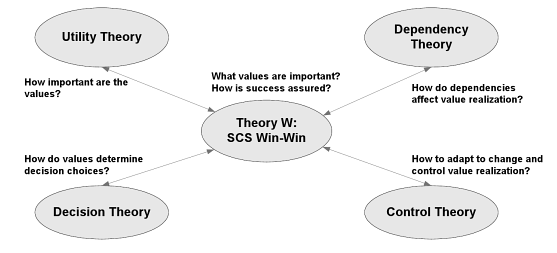
\includegraphics[scale=0.6]{4+1theorem}
\label{fig:fouronetheorem}
\end{figure} 

The essence of VBSE and were it distinguish itself from the previous processes and strategies is that it does not operate with the same values-neutral approach. Where previous strategies treated every requirement, use case or defect with equal importance the VBSE seek to find a mutually satisfactory set of objectives for SCS' and company, and work these into a system.

This way of thinking manifests itself in a number of activities, which tries to maximize the value created on different levels of the engineering practices.
These activities are:
\begin{itemize}
\item Value-based Requirement Engineering
\item Value-based Architecting
\item Value-based Design and Deployment
\item Value-based Verification and Validation
\item Value-based Planing and Controlling 
\item Value-based Risk Management
\item Value-based People Management
\item Value-based Principles and Practices addressing
\item Value-based Quality Management
\end{itemize} 

\paragraph{Quality management in VBSE}
Quality management in VBSE is focussing on prioritizing desired quality factors with respect to the stakeholders' value propositions. A crucial part of the quality management in VBSE is to identify what these factors are. Since software quality is multidimensional, it follows that the quality of a system can acceptable in one situation is not in odder. For instance a making a system with high efficiency but unknown or low reliability might be sufficient for a smart phone game application but as a system for a security system for a space program it is a no go. Further since quality costs money, narrowing down the which qualities really are important for stakeholders is a way to reduce wasted effort and money. In VBSE the quality management is concerned with identifying the most important qualities which should characterize the system and making sure that these are achieved to the extend where it meets the requirements of the stakeholders and no more. 
The main problem in VBSE is how to find out which quality factors are important, to which extend they should be meet. 

Further it is a problem in VBSE to verify that the quality goal identified is actually the correct once. Having a cap between the identified desired quality need and the \textit{true} quality need can lead to a business failure. 
Traditional development proposes to make studies of the user and the environment of the system to give evidence for a verification or rejection of a set of quality goal. But these studies can be costly and misleading, since the user does not always know what they want. Nor does a assessment of the environment prof whether one solution is better than another. Without any hard evidence, quality management in VBSE and other strategies can be a nasty business. Continuous Experimentation can be applied in this situation to reduce this risk of having wrong quality requirement. 

\subsection{Continuous Experimentation}
Continuous Experimentation is a development approach which uses both Value-oriented software development and Continuous delivery. 

\subsubsection{Hypothesis}
The first step in order to define a task in continuous experimentation is defining the requirements for the experiment to succeed. 

In order to succeed the experiment has to bring value to the product. In order to measure how well the experiment perform a hypothesis which describe an expected outcome from the experiment.

The core of the hypothesis has to be quality requirements, which can be tested and verified in order to verify the value of the experiment to the product. 

The Hypothesis has to be developed into a Minimal Viable Product, which will be the tested component for analysis.

\subsubsection{Data Analysis}
Once the minimal viable product has been deployed into production. Users are monitored and data about the users and their behavior is collected for analysis of how the change has affected the product. 

This process require data scientist in order to  analyze the benefits and consequences of the experiment upon the product. 

\subsubsection{Validation}


\section{Discussion}

\subsection{Consequences of Value-oriented Software Development}
\subsection{Synergy of CX and VoSD}
\subsection{Profit!}

\section{Conclusions}
%\end{document}  % This is where a 'short' article might terminate

%ACKNOWLEDGMENTS are optional
\section{Acknowledgments}

After all Coffee isn't that bad 

%
% The following two commands are all you need in the
% initial runs of your .tex file to
% produce the bibliography for the citations in your paper.
\bibliographystyle{abbrv}
\bibliography{sigproc}  % sigproc.bib is the name of the Bibliography in this case
% You must have a proper ".bib" file
%  and remember to run:
% latex bibtex latex latex
% to resolve all references
%
% ACM needs 'a single self-contained file'!
%
%APPENDICES are optional
%\balancecolumns


\end{document}
